\chapter{Библиотека TopicNet и её применение в конкретных задачах} 

% “Мы подготовили рецепт: мы берём комбинацию регуляризаторов, и оно почти всегда работает хорошо из коробки”

Данный раздел будет посвящён библиотеке TopicNet. TopicNet -- открытая надстройка над библиотекой BigARTM, предоставляющая более удобные возможности  для подбора гиперпараметров, для работы с пользовательскими регуляризаторами и для визуализации тематических моделей \cite{bulatov2020topicnet}.  

Описанная библиотека доступна онлайн на GitHub\footnote{\url{github.com/machine-intelligence-laboratory/TopicNet}}, также опубликована её документация \footnote{\url{machine-intelligence-laboratory.github.io/TopicNet} }.  

\section{Сравнимые проекты} 

% Given a generative model and data, inference must be executed for extracting probabilistic topic-depending distributions. There are many inference algorithms: expectation-maximization (EM) algorithm, Gibbs sampling, variational inference, gradient descent and message passing. In ARTM the regularized EM-algorithm is used to learn model parameters. The similarities between each of the algorithms were noted before in \cite{asuncion09smoothing}.  

Gensim \cite{rehurek_lrec} --- наиболее популярный фреймворк для тематического моделирования. В нём реализован ряд известных моделей (LSA, pLSA, LDA, Hierarchical Latent Dirichlet Allocation (HLDA) и их производные). Также эта библиотека предоставляет интерфейс измерения когерентности по верхним токенам темы, основанный на работе \cite{roder2015exploring}. Gensim написан на языке Python и оптимизирован для работы с большими коллекциями документов.  

Stanford Topic Modelling Toolbox~--- STMT \cite{stanfordtmt}, написанный на Scala, поддерживает обучение LDA, Labelled LDA и PLDA. Полезной особенностью Stanford TMT является интеграция с Excel.  

MALLET \cite{mccallum2002mallet} --- классическая реализация тематического моделирования, написанная на Java и основанная на сэмплировании Гиббса. Инструментарий MALLET позволяет строить модели LDA, Pachinko Allocation \cite{li2006pachinko}, и HLDA. Часто используется для онлайн-сервисов \cite{pol2017towards}.  

A Library of Short Text Topic Modelling (STTM) \cite{qiang2018sttm} ~--- написанный на Java фреймворк, предназначенный для работы с коллекциями коротких текстов. Данный пакет поддерживает множество специализированных моделей: Dirichlet Multinomial Mixture DMM \cite{yin2014dirichlet}, Word Network Topic Model WNTM \cite{zuo2016word}, Pseudo-Document-Based Topic Model PTM \cite{zuo2016topic} and Self-Aggregation-Based Topic Model SATM \cite{quan2015short}. Также поддерживаются некоторые модели, предназначенные для работы с длинными текстами: LDA и Latent Feature Model with LDA \cite{nguyen2015improving}.  

Familia \cite{jiang2018familia} --- фреймворк, поддерживающий LDA и Supervised LDA: Topics Over Time TOT \cite{wang2006topics}, Bilingual Topic Model \cite{gao2011clickthrough}, Location-Aware Topic Model LATM \cite{wang2007mining}. Авторами было заявлено, что Familia даёт возможность <<проектировать свои собственные тематические модели>>, используя сэмплирование Гиббса как механизм вывода. К сожалению, репозиторий на GitHub такую функцию не поддерживает: в открытом релизе отсутствует возможность построить пользовательскую тематическую модель и даже возможность обучить представленные модели на пользовательской коллекции \cite{familia_github}.  

Библиотека \texttt{TOM} для Python\footnote{ https://github.com/AdrienGuille/TOM} поддерживает LDA и модели, основанные на неотрицательном матричном разложении \cite{guille2016tom}. Пакет \texttt{ldatuning} для R позволяет строить модели LDA и CTM \cite{ldatuning}. Оба этих проекта интересны тем, что в них реализован ряд критериев качества, описанных в \ref{chap:metrics}, и используют их для подбора числа тем $T$.  

Как было отмечено выше, высокий порог входа в область тематического моделирования для потенциальных пользователей по-прежнему остаётся важной проблемой, которую необходимо решить. Ситуация ещё более осложняется, если пользователю необходимы не классические модели, доступные в самых популярных фреймворках (Gensim, MALLET), а более продвинутые их модификации.  

Другой аспект этой проблемы --- построение новых тематических моделей с нуля. Самостоятельно реализовать классические тематические модели сравнительно несложно и доступно любому пользователю с навыками программирования. Однако эффективное построение комплексных многокритериальных моделей требует больших затрат времени и усилий (при этом трудно гарантировать вычислительную эффективность и отсутствие программных ошибок) \cite{jiang2018familia}.  

Цель библиотеки TopicNet --- сделать имеющийся инструментарий тематического моделирования более доступным для широкой публики и облегчить конструирование новых тематических моделей.  

% Due to ARTM formalism, TopicNet offers natural language processing community access to Python-based multimodal topic modelling that supports large documents and huge corpora.  

\section{Технология в основе} 

Библиотека TopicNet --- это высокоуровневая надстройка над библиотекой BigARTM. Мы более детально рассмотрим плюсы библиотеки \mbox{BigARTM} и её минусы, которые мы надеемся компенсировать посредством библиотеки TopicNet.  

\subsection{Достоинства BigARTM} 

% ### CHANGE ### 

BigARTM --- быстрая и гибкая библиотека для тематического моделирования \cite{frei2016parallel}, основанная на формализме Additive Regularization of Topic Models (ARTM) \cite{vorontsov2014additive}. Идея подхода состоит в том, чтобы перейти от оптимизации правдоподобия к оптимизации регуляризованного правдоподобия (используя модифицированный EM-алгоритм).

Регуляризация выполняет две цели. Во-первых, она обеспечивает устойчивость за счёт накладывания дополнительных ограничений на решение. Во-вторых, каждый дополнительный регуляризатор позволяет указать на желательность каких-либо дополнительных свойств модели: например, разреженность распределений, различность тем, когерентность верхних токенов.  

Также регуляризация может учесть какую-то дополнительную информацию. Чаще всего встречающийся на практике случай --- использование метаданных документа (e.g. authors, timestamps, tags, and n-grams). Воспользоваться этой информацией в рамках подхода АРТМ оказывается существенно проще, чем в байесовых подходах: правдоподобие каждой дополнительной модальности можно рассматривать как регуляризатор, аддитивно применённый к тематической модели над множеством слов \cite{voron15nonbayesian}.  

Список работ, использующих гибкость ARTM и BigARTM, включает в себя: улучшение качества разведочного поиска \cite{yanina17technews}, построение интерпретируемых тематических представлений слов посредством модели сети слов \cite{potapenko17interpretable}, иерархическое тематическое моделирование \cite{chirkova2016additive}, улучшение представлений документов для задач текстовой регрессии \cite{sokolov15topic}, нахождение редких этнорелевантных тем в социальных сетях \cite{apishev16additive,apishev16mining}, использование лингвистических признаков \cite{popov_hier}, отбор тем при помощи разреживающей энтропийной регуляризации \cite{voron15plavin}, улучшение тем при помощи сегментации текста \cite{skachkov}, прямая оптимизация когерентности верхних токенов \cite{4keys}, отход от гипотезы мешка слов за счёт использования определённой метрики качества \cite{intracoh}.

Обзор \cite{kochedykov2017fast} показывает, как байесовы тематические модели (в том числе multimodal, multilingual, temporal, hierarchical, graph-based, and short-text topic models) могут быть переформулированы в терминах подхода АРТМ.  

Разработка как теории АРТМ, так и библиотеки \mbox{BigARTM} продолжается и по сей день. Многие существующие регуляризаторы были вкладом со стороны сообщества.  

Насколько нам известно, по гибкости BigARTM превосходит все остальные фреймворки для тематического моделирования. Из перечисленных выше аналогов лишь Familia заявляет о сравнимом функционале; при этом в открытом релизе Familia такой функционал отсутствует \cite{familia_github}.  

\subsection{Недостатки BigARTM} 

Оптимизации, направленные на вычислительную эффективность, делают BigARTM мощным инструментом, который, однако, имеет ограниченную область применимости. Если пользователь уже имеет точное описание требуемой регуляризованной модели, то библиотека BigARTM способна очень быстро выучить её параметры $\Phi$, $\Theta$. К сожалению, наличие таких готовых спецификаций --- редкость.  

Число тем --- самый распространённый среди различных тематических моделей гиперпараметр. Все средства для тематического моделирования предоставляют пользователю возможность указать этот гиперпараметр; большинство из них не дают никаких рекомендаций по выбору хорошего значения. Много работ посвящено этому вопросу.  

В подходе АРТМ ситуация ещё более ухудшается; действительно, теперь пользователь может скомбинировать произвольное число регуляризаторов, каждый из которых имеет индивидуальный коэффициент регуляризации (а также, возможно, какие-либо другие структурные параметры). Всё вышеуказанное никак не регламентируется.  

Второй фактор, увеличивающий порог входа, --- некоторое неудобство интерфейса библиотеки. Это естественный итог того, что новый экспериментальный функционал разрабатывался и встраивался в библиотеку до того, как сообществом были выработаны "лучшие практики" по его применению (а также желания сохранить обратную совместимость).  

% Так получается парадоксальный результат: Therefore, as applications of \mbox{BigARTM} were becoming more diverse and the algorithms were gradually refined, the high-level interface of \mbox{BigARTM} was getting less well-suited for <<best practices>>.  

Ещё одна проблема библиотеки BigARTM --- сложность её расширения. С технической точки зрения, библиотека BigARTM состоит из высокопроизводительного ядра, написанного на \cpp и ряда классов-обёрток на языке Python. Реализованные на \cpp низкоуровневые функции тщательно оптимизированы, многопоточны --- всё это даёт BigARTM превосходство в скорости. С другой стороны, это затрудняет понимание и изменение данного фундаментального низкоуровневого кода. Высокоуровневый интерфейс не всегда предоставляет достаточную гибкость (например, для испытаний пользовательских регуляризаторов) 

\section{Мотивация и видение} 

Главная мотивация TopicNet --- создать инструмент, удобный как для новичков, так и для продвинутых пользователей. Эти две группы пользователей не обязаны использовать библиотеку одним и тем же образом; важнее всего обеспечить возможность взаимодействия групп друг с другом. Нами был сформулирован ряд требований, необходимых для достижения этой цели: 

\begin{itemize}

\item{Модулярность: библиотека должна быть организована как совокупность независимых блоков, каждый из которых можно использовать в отрыве от остальных. Это требование обусловлено двумя причинами. Во-первых, это упрощает переход на новую технологию: продвинутые пользователи могут получить какую-либо пользу от использования TopicNet, не внося радикальных правок в существующие проекты. Во-вторых, это необходимо для создания активного сообщества пользователей и разработчиков TopicNet: программные проекты с понятной структурой более привлекательны для участников-контрибьюторов.} 
\item{Инструменты визуализации: библиотека должна предоставлять пользователю набор мощных инструментов для визуализации.  Такие инструменты играют важную роль при отладке и анализе ошибок, а также могут быть полезны для итоговых прикладных задач (например, показ похожих документов может быть нужен для отладки или непосредственно быть костяком системы разведочного поиска).  Согласно вышеописанному требованию модулярности, этот инструментарий должен быть самодостаточным и иметь возможность развиваться в отрыве от остальной кодовой базы TopicNet.} 
\item{Краткость: библиотека должна скрыть от пользователя низкоуровневые детали, давая возможность сосредоточиться на более существенных проблемах. Важно улучшить творческий процесс построения модели для решения конкретной задачи.  Второе соображение в пользу этого решения основывается на принципе <<Соглашения по конфигурации>> (<<convention over configuration>>). Уменьшая количество вещей, требующих явной настройки, и предоставляя разумные значения по умолчанию, можно <<привить>> пользователю принятые в сообществе лучшие практики (такие как сохранение построенных моделей или хранение данных для разных коллекций в разных директориях).  Третье преимущество заключается в читаемости и портируемости. Работая с более сжатым и регулярным кодом, пользователь может видеть бо'льший объём кода в рамках экрана, что улучшает понимание эксперимента. В результате становится легче обсуждать, изучать и отлаживать эксперименты, а также делиться ими.} 
\item{Работа <<из коробки>>: в состав библиотеки должны входить схемы тренировки моделей, готовые к использованию и дающие приемлемый результат. Эти схемы должны подытоживать найденные сообществом стратегии решения определённых задач. Это обеспечивает пользователю-новичку положительный опыт первого взаимодействия с библиотекой и предоставляет продвинутому пользователю средство компактной записи для своих наработок.} 
\end{itemize}

\section{Архитектура} 

Библиотека TopicNet состоит из двух больших модулей: \texttt{viewers} и \texttt{cooking machine}.  

Модуль \texttt{Viewers} содержит различные инструменты визуализации. Дизайн придерживается философии Unix: каждый вьювер имеет ограниченную область ответственности и способен возвращать результат операции в JSON-подобном виде.

Это даёт возможность комбинировать содержащиеся в модуле вьюверы, не теряя при этом удобные для конечного пользователя методы, возвращающие \texttt{pandas.DataFrame}, строку сформированного HTML, или отображающие результат сразу в ячейке вывода Jupyter Notebook. Примеры вывода TopTokensViewer и DocumentClusterViewer приведены на Рис. \ref{top_tokens} и \ref{documents_clusters} соответственно.  

\begin{figure*}[h]
    \centering
    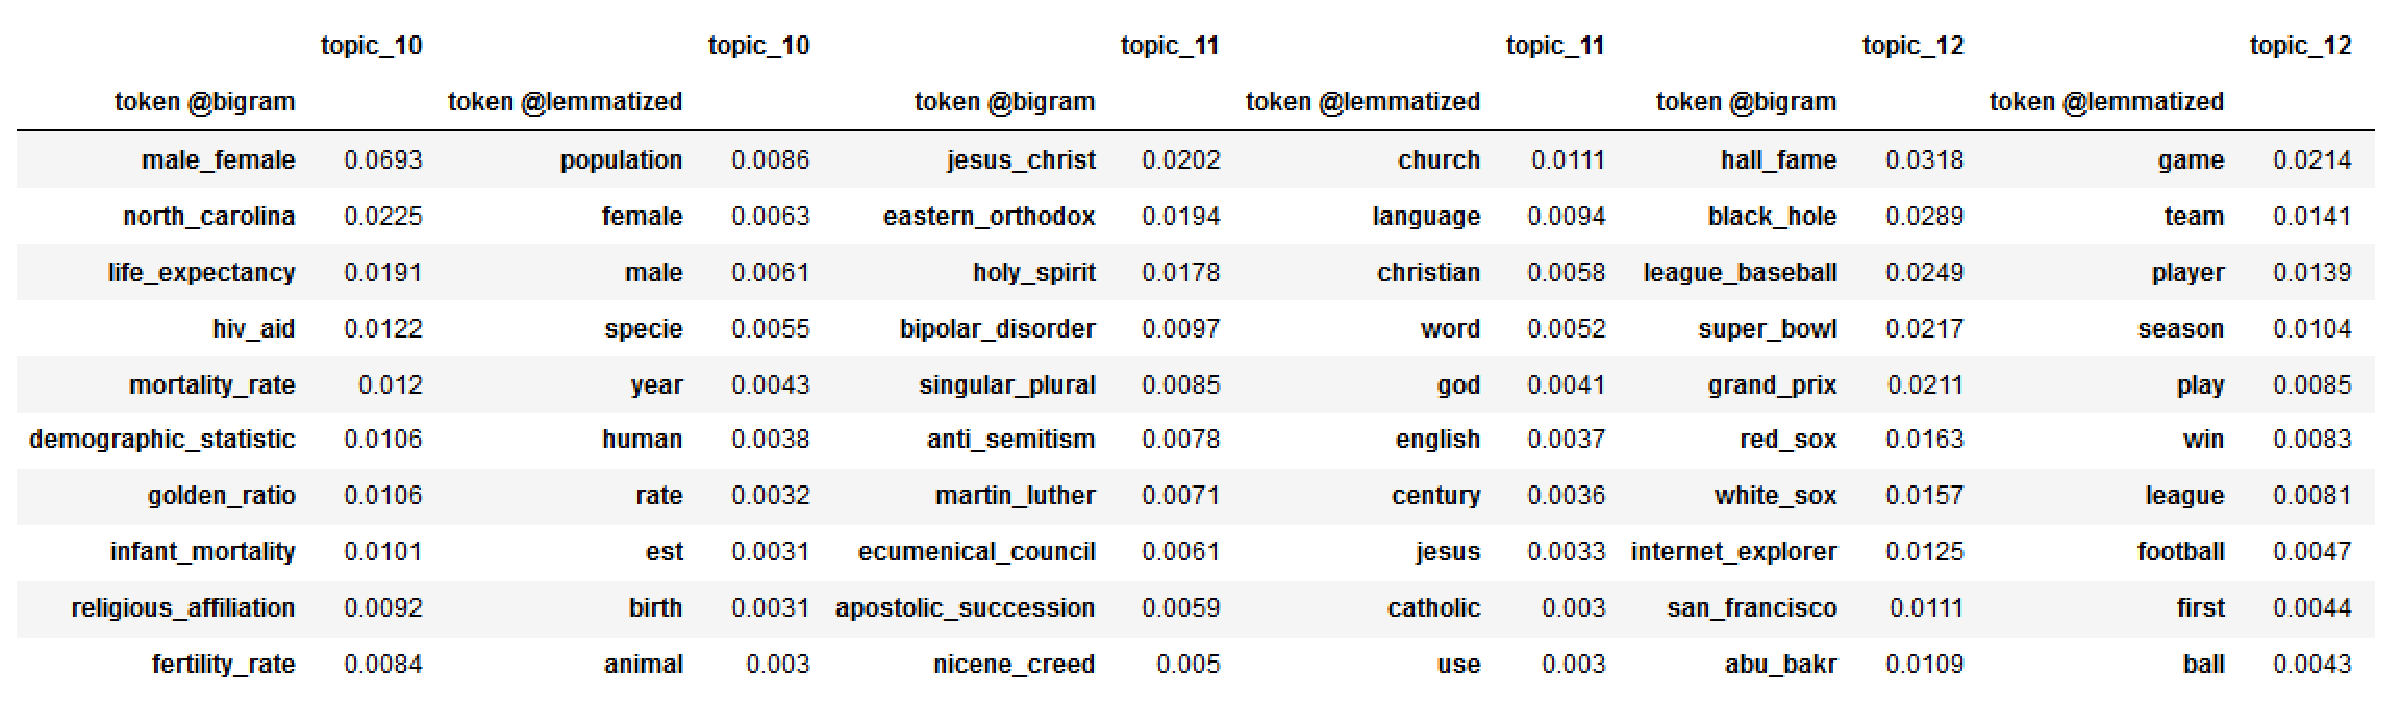
\includegraphics[width=0.98\textwidth]{sorted_3_topics.eps}
    \caption{Вывод TopTokensViewer. Для каждого токена вычисляется заданная функция, используемая для сортировки и выбора токенов для показа. Функция здаётся при инициализации вьювера.}
\label{top_tokens}
\end{figure*} 

\begin{figure}[h]
    \centering
    \includegraphics[width=0.5\textwidth]{cluster_plot.eps}
    \caption{Визуализация документов после понижения размерности посредством DocumentClusterViewer. Цвет каждой точки связан с темой соответствующего документа.}
\label{documents_clusters}

\end{figure} 

% Examples? common tasks such as TopTokenViewer and TopDocumentViewer and more sophisticated ones like SimilarDocumentViewer, TopicSpectrumViewer 

% The library supports a variety of visualisation tools both conventional, such as top tokens and top documents viewers, and experimental ones.  

Модуль \texttt{Cooking Machine} содержит различные инструменты для моделирования, расположенные в иерархии основных классов. Эти классы отвечают за построение и обучение модели заданной структуры, за отбор моделей согласно заданным пользователем ограничениям, а также за сохранение, загрузку и журналирование происходящего процесса.

Следуя вышеописанному принципу <<соглашения по конфигурации>>, мы накладываем ряд ограничений на вид экспериментов, которые может провести пользователь.

Мы исходим из допущения о том, что процесс построения тематической модели представим в виде дерева. Каждый узел дерева содержит в себе тематическую модель, а ориентированные рёбра хранят информацию об отношениях <<предок-потомок>> вида <<модель $Y$ была получена из модели $X$ при помощи преобразования $T_{XY}$>>. Не все деревья эксперимента являются допустимыми. Мы накладываем ограничения на допустимые преобразования: требуем, чтобы все рёбра одного уровня описывали преобразования из одного и того же семейства, различающиеся лишь набором параметров.  

Возможные примеры таких преобразований: 

\begin{itemize}
    \item Применить к модели регуляризатор с произвольными параметрами (или изменить параметры существующего регуляризатора)
    \item Запустить процесс обучения модели на какое-то количество итераций
    \item Добавить в текущую модель несколько тем, обнаруженных внутри другой коллекции
\end{itemize} 

\begin{figure}[t]
    \centering
    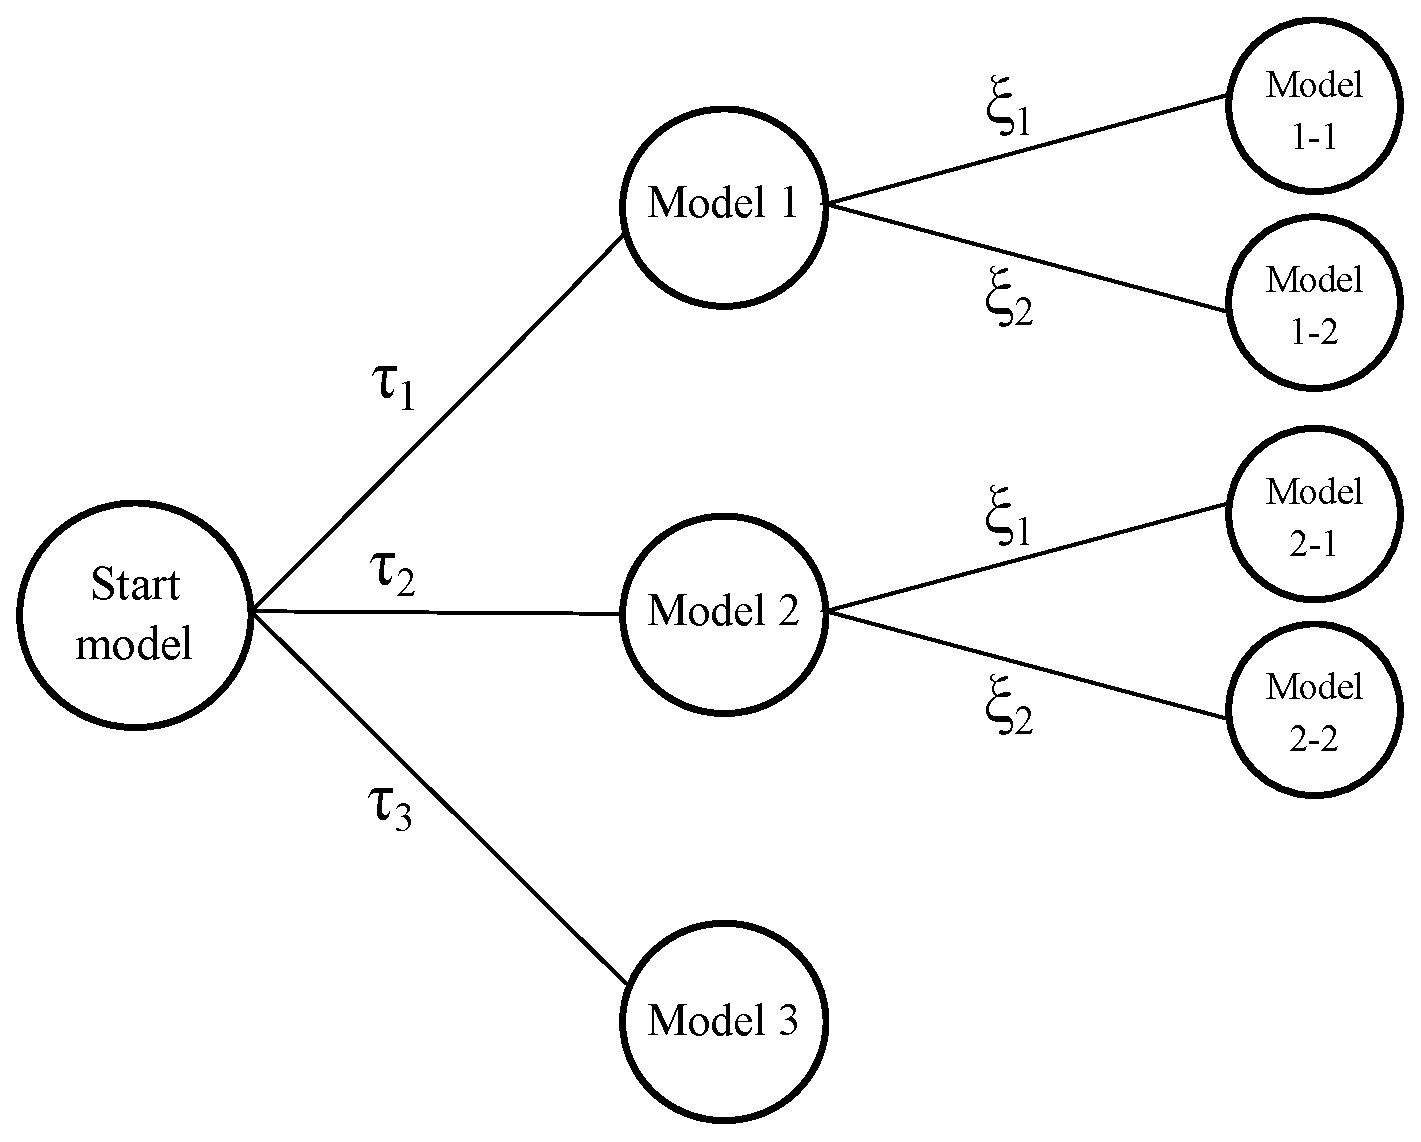
\includegraphics[width=0.4\textwidth]{training_scheme_example.eps}
    \caption{
        Пример двухэтапной схемы эксперимента.
        На первом этапе применяется регуляризатор с коэффициентом $\tau$, принимающим значения из некоторого множества $\{\tau_1, \tau_2, \tau_3\}$.
        Лучшими моделями после первого этапа являются \emph{Model 1} и \emph{Model 2}, поэтому \emph{Model 3} больше не участвует в процессе обучения.
        Второй этап связан с другим регуляризатором с коэффициентом $\xi$, принимающим значения из множества $\{\xi_1, \xi_2\}$.
        В результате этого этапа у каждой из ранее отобранных моделей  появляется два потомка.}
\label{Training-scheme}
\end{figure} 

Класс \texttt{Experiment} отвечает за хранение, журналирование и актуализацию этой структуры.  

Все преобразования связаны с экземпляром класса \texttt{Cube}. Каждый \texttt{Cube} играет роль чертежа, задающего все преобразования на текущем уровне эксперимента. Таким образом, процесс обучения можно представить как цепочку кубов, последовательно соединённых друг с другом.  

Куб выполняет две важные функции. Первая --- это \textit{спецификация}: во время инициализации куб преобразует заданные пользователем параметры в многомерное пространство поиска. Вторая функция --- \textit{применение}: получив точку в пространстве поиска и тематическую модель, куб изменяет какое-либо количество параметров и/или гиперпараметров модели. Таким образом, он играет роль инкубатора для моделей, что отражено в названии класса. На Рис.  \ref{Training-scheme} приведена схема обучения, состоящая из двух кубов, применённых к одной модели.  

Классы \texttt{Experiment} и \texttt{Cube} позволяют сделать логгирование и сложные стратегии обучения более сжатыми и доступными. Модуль \texttt{config\_parser} делает ещё один шаг в сторону облегчения конфигурируемости: стратегию обучения можно задать при помощи текстового конфигурационного файла в формате YAML.  

\section{Механизм отбора моделей в TopicNet} 

\begin{figure*}[!ht]
\footnotesize
\texttt{TopicKernel@word.average\_contrast > 0.95 * MAXIMUM(TopicKernel@word.average\_contrast) \\
\hphantom{\ \ } and PerplexityScore@all < 1.1 * MINIMUM(PerplexityScore@all) \\
\hphantom{\ \ } and SparsityPhiScore@word -> max\\
\hphantom{\ \ } COLLECT 3}
\caption{Пример строки, задающей критерий отбора моделей. Здесь в качестве критериев отбора участвуют перплексия, контраст лексического ядра модальности \texttt{@word} и разреженность матрицы $\Phi$. Результатом будут три модели, контраст которых не более чем на 5\% отличается от наилучшего достигнутого контраста, имеют допустимую перплексию и как можно более разреженны.}
\label{DSL-example}
\end{figure*} 

Другая область, описываемая пользователями как громоздкая и непрозрачная, --- отбор моделей. В реальных экспериментах не у каждой модели есть потомки; большинство моделей отбрасывается в соответствии с каким-то критерием. Самый естественный, но в то же время самый трудозатратный способ --- это ручное изучение список верхних токенов и верхних документов, на основании которого пользователь принимает решение, какие из моделей являются <<удовлетворительными>>. Другой подход заключается в сравнении численных показателей; обычно используется перплексия и когерентность. Библиотека \mbox{BigARTM} добавляет к их числу ещё какое-либо число дополнительных метрик: например, разреженность, чистота и контраст \cite{voron15mlj}.  

Библиотека TopicNet также поддерживает пользовательские критерии качества. Значительная часть мер, описанных в \ref{chap:metrics}, реализована на платформе TopicNet.  

Для того чтобы облегчить груз ручной инспекции, мы реализовали простой domain-specific язык для отбора моделей (пример приведён на Рис \ref{DSL-example}). Результатом этого становится более простой и прозрачный процесс отбора моделей, способный учитывать множество критериев одновременно.  

В рамках описываемого подхода каждый критерий отбора моделей представляет собой строку текста на языке, который может быть задан следующей контекстно-свободной грамматикой: 

\begin{lstlisting}

S -> <Expr> | <Expr> <Clct>

<Clct> -> COLLECT <Int>

<Expr> -> <Expr> AND <Expr>

<Optr> -> less | eq | great

<Expr> -> <Literal> <Optr> <Number>

<Expr> -> <Literal> to MIN | <Literal> to MAX

<Literal> -> <ScoreName> | model<ParameterName>

\end{lstlisting} 

Будем называть выражения вида

\lstinline{<Literal> <Optr> <Number>} \textit{требованиями}, а выражения вида \lstinline{<Literal> to MIN} и \lstinline{<Literal> to MAX} --- \textit{критериями}. \textit{MIN} и \textit{MAX} задают направление улучшения (вернуть модель с наименьшим либо с наибольшим значением).  

Здесь \lstinline{<Int>} обозначает любое неотрицательное целое число, а \lstinline{<Number>} может быть целым числом, дробным числом либо арифметическим выражением, использующим специальные функции \texttt{MINIMUM}, \texttt{MAXIMUM}, \texttt{AVERAGE}, \texttt{MEDIAN}.  

Символ \lstinline{<ScoreName>} означает имя критерия качества (скора модели, например разреженности), а \lstinline{<ParameterName>} --- свойство тематической модели (например, число тем: \texttt{model.num\_topics}). Требования, содержащие \lstinline{<ParameterName>}, будем называть \textit{структурными требованиями}.  

Специальные функции \texttt{MINIMUM}, \texttt{MAXIMUM}, \texttt{AVERAGE}, \texttt{MEDIAN} применяются к \lstinline{<Literal>} (например, \texttt{MINIMUM(model.num\_topics)} или \texttt{MEDIAN(SparsityThetaScore)}). В процессе программной обработки эти функции заменяются на их численные значения, что позволяет использовать требования вида \texttt{SparsityPhiScore\@word > MEDIAN(SparsityPhiScore\@word)} наряду с более простыми \texttt{SparsityPhiScore\@word > 0.8}.  

Сам процесс отбора происходит в несколько этапов. Сначала выбираются все модели, удовлетворяющие заданным структурным требованиям (если структурных требований не задано, то выбираются все модели). Затем по полученной выборке рассчитываются значения специальных функций, после чего на основании не-структурных требований формируется следующий набор моделей. Если критерий отбора не задан, то этот набор просто возвращается пользователю. 

Если же критерий отбора задан, то этот набор упорядочивается согласно данному критерию. Если

имеется дополнительная клауза \texttt{COLLECT N}, то результатом работы будут $N$ наилучших моделей; иначе считается, что $N=1$.  

\section{Сравнение с конкурентами} 

Сравнение TopicNet с другими фреймворками затрагивает несколько важных аспектов. Во-первых, нужно было убедиться в том, что обучение одной модели не занимает слишком много времени и не требует слишком много ресурсов. Во-вторых, нужно оценить интерпретируемость и различность тем у каждой модели.  

Эксперименты проводились на коллекции 20 newsgroups. По набору 10 верхних токенов каждой темы измерялись две характеристики:

\begin{itemize}
    \item Umass-когерентность, показывающая согласованность слов между собой. Измерение производилось при помощи сервиса Palmetto \footnote{\url{palmetto.aksw.org/palmetto-webapp} } \cite{roder2015exploring}. В предыдущих работах было показано, что когерентность коррелирует с интерпретируемостью тем \cite{mimno2011}.
    \item Коэффициент подобия Жаккара, показывающий различность полученных тем. Коэффициент подобия, равный нулю, означает, что в верхних словах тем нет общих слов (то есть множества их верхних 10 токенов не пересекаются), а равенство его единицы означает, что все темы являются полными дубликатами.
\end{itemize} 

\subsection{Использование ресурсов} 

Использование вычислительных ресурсов является фактором, который может затруднить широкое распространение фреймворка (например, студенты могут не иметь доступа к большим вычислительным мощностям; промышленное  использование также требует высокой скорости работы и низкой нагрузки на машину). Это сравнение будет проводиться на более крупном датасете NIPS \cite{mccallum1996bow}.  

\begin{table}[h]
\begin{tabular}{|l|l|l|}
\hline
                      & \multicolumn{1}{c|}{RAM, MB} & \multicolumn{1}{c|}{Training time, s} \\ \hline
TopicNet              & 991                         & 222.6 (15)                             \\ \hline
TopicNet multiprocess & 1084                        & 51.4 (15)                              \\ \hline
Gensim LDA            & 3559                        & 282.3 (3)                              \\ \hline
STTM DMM              & 3202                        & 52997 (1)                              \\ \hline
STTM PTM              & 1604                        & 84677 (1)                              \\ \hline
STTM WNTM             & 18663                       & 157819 (1)                             \\ \hline
\end{tabular}
\caption{Сравнение различных реализаций тематического моделирования по расходу вычислительных ресурсов. В первом столбце приведен максимальный объём оперативной памяти, занятой процессом во время обучения. Второй столбец показывает время, затраченное на обучение суммарно и количество построенных моделей (из которых отбирается лучшая).}
\label{performance-benchmark}
\end{table} 

Как видно из таблицы \ref{performance-benchmark}, даже однопоточная версия превосходит конкурентов в скорости; использование нескольких процессоров незначительно увеличивает расход оперативной памяти, но намного ускоряет процесс обучения. Таким образом, TopicNet не добавляет слишком много дополнительных накладных расходов по сравнению с чистой библиотекой BigARTM.  

\subsection{Model Quality} 

Следуя изложенным выше целям, мы предоставляем рецепт \texttt{ARTM baseline}, предназначенный для знакомства с библиотекой. Чтобы проверить качество этого рецепта, мы сравним модель, полученную посредством рецепта \texttt{ARTM baseline} с моделями <<по умолчанию>> из других фреймворков. Модели LDA и STTM были построены на 20 темах, модель TopicNet состояла из 19 предметных тем и одной фоновой. Никакой дополнительной настройки гиперпараметров не производилось (код тренировки модели приведён на \ref{topicnet_baseline}).  

% for TopicNet model we set 19 topics and one <<background>> topic, which has a special set of regularizers to collect polythematic documents.  

\begin{figure}[!ht]
    \centering
    \includegraphics[width=0.4\textwidth]{topicnet_baseline.eps}
    \caption{Пример базового эксперимента в TopicNet.}
\label{topicnet_baseline}
\end{figure} 

\begin{table}[h]
\begin{tabular}{|l|l|l|}
\hline
           & \multicolumn{1}{c|}{\begin{tabular}[c]{@{}c@{}}Jaccard measure\\ of topic dissimilarity\end{tabular}} & \multicolumn{1}{c|}{\begin{tabular}[c]{@{}c@{}}Average topic\\ coherence\end{tabular}} \\ \hline
TopicNet   & \textbf{0.00169}                                                                                               & -2.551                                                                                 \\ \hline
Gensim LDA & 0.01374                                                                                               & -2.747                                                                                 \\ \hline
STTM DMM   & 0.37541                                                                                               & -2.726                                                                                 \\ \hline
STTM PTM   & 0.02485                                                                                               & \textbf{-2.510}                                                                                 \\ \hline
STTM WNTM  & 0.01997                                                                                               & -3.572                                                                                 \\ \hline 
\end{tabular}
\caption{Topic quality comparison}
\label{topic-comparisson}

\end{table} 

Как мы видим из таблицы \ref{topic-comparisson}, построенная TopicNet модель  оказывается на втором месте по интерпретируемости (рис. \ref{topics_distribution} показывает дополнительную информацию о когерентности) и на первом месте по критерию различности тем. Это объясняется регуляризатором декорреляции, используемым в рецепте \texttt{ARTM baseline}. Комбинация этого регуляризатора, используемого скора и механизма, следящего за повышением перплексии, позволила найти модель, удовлетворяющую несколько требований одновременно.  

\begin{figure}[!ht]
    \centering
    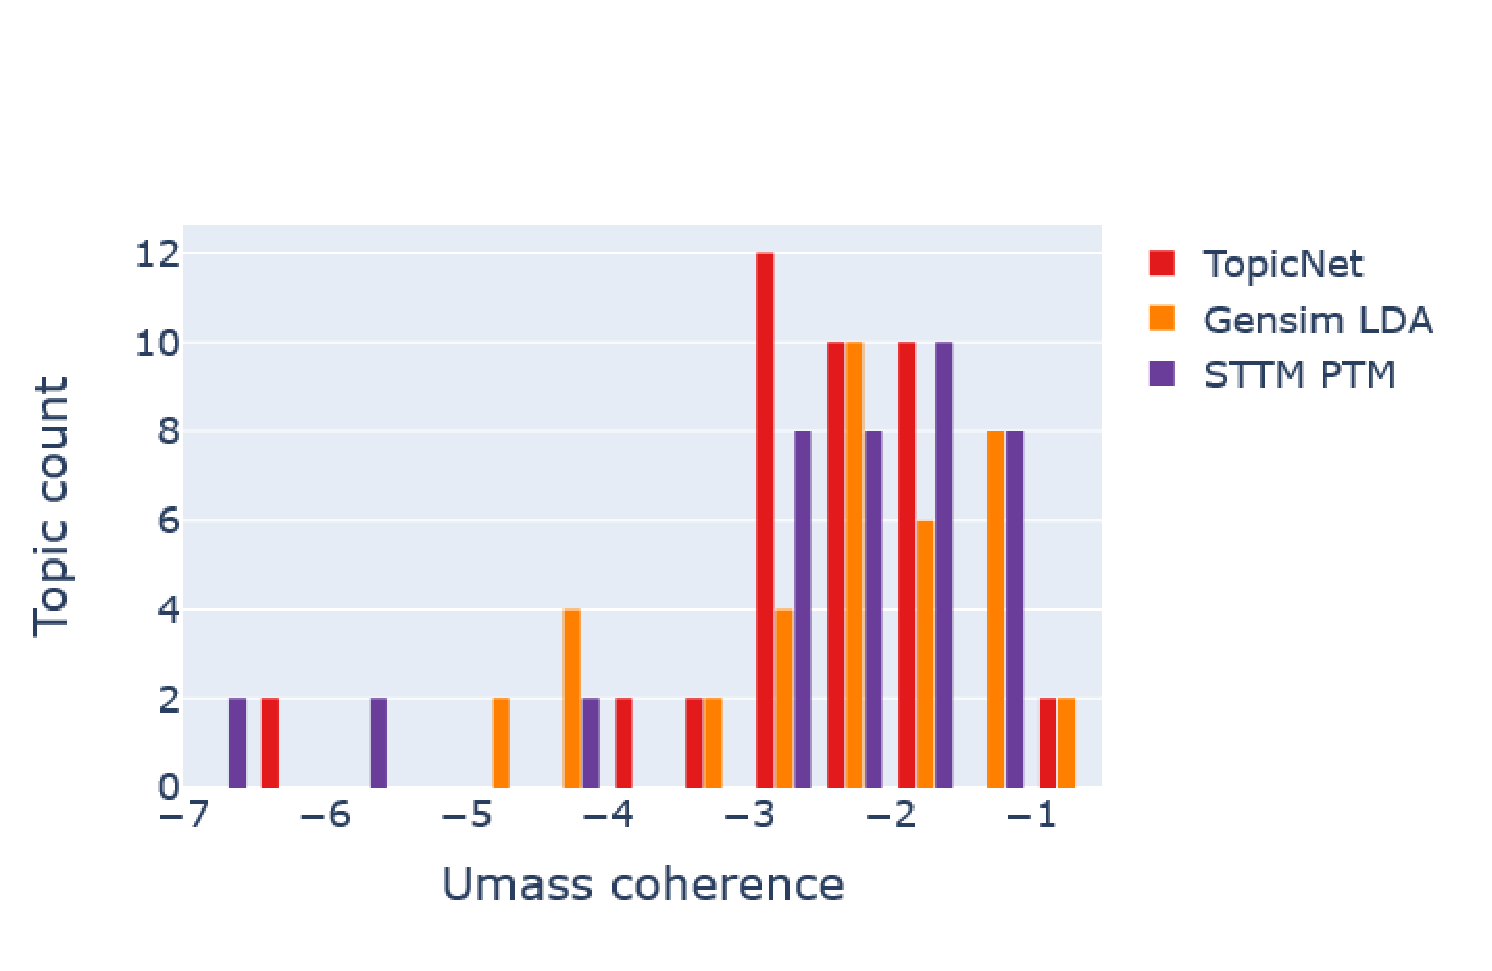
\includegraphics[width=0.45\textwidth]{Topics.eps}
    \caption{Распределение когерентности тем.}
\label{topics_distribution}
\end{figure} 

\subsection{Использование псевдорегуляризатора быстрой векторизации} 

Во второй серии экспериментов проводилось более детальное сравнение TopicNet с GenSim на той же коллекции.  

У GenSim есть несколько режимов запуска, которые можно описать как <<параметры по умолчанию>>. Величина $\alpha_{td}$, задающая априорное распределение на $\Theta$, может принимать значения \texttt{asymmetric}, \texttt{symmetric}, \texttt{auto}. Аналогичные значения (кроме \texttt{asymmetric}) может принимать и величина $\eta_{wt}$, задающая априорное распределение на $\Phi$.  В GenSim инициализация LDA симметричным и/или асимметричным способом задаёт фиксированный численный вектор. Опция \texttt{auto} ведёт себя иначе: параметры распределения Дирихле будут обновляться в процессе обучения модели при помощи метода Ньютона \cite{huang2005maximum}.  

Эти шесть моделей на базе GenSim будут сравниваться с тремя моделями, полученными средствами библиотеки TopicNet. Первая модель --- результат работы рецепта \texttt{BaselineRecipe} (в котором настраивалось только число тем): 

\begin{itemize}
    \item Количество тем в модели: 20 предметных, 1 фоновая;
    \item Два регуляризатора сглаживания фоновых тем по $\Phi$ и $\Theta$ с относительным коэффициентом $\tau=0.1$;
    \item Регуляризатор декорреляции с неизвестным относительным коэффициентом $\tau$ воздействует на предметные темы;
    \item Перебор коэффициента декорреляции $\tau$ производится при помощи \texttt{RegularizersModifierCube} с шагом $0.01$ (стартовое значение $0$, остановка происходит, если перплексия текущей модели более чем а $5\%$ превосходит перплексию модели с $\tau=0$);
    \item Критерий отбора модели: \texttt{PerplexityScore@all < 1.05 * MINIMUM(PerplexityScore@all) and BleiLaffertyScore -> max}.
\end{itemize} 

Результатом этого процесса является тематическая модель с коэффициентом декорреляции $\tau=0.09$. Две другие модели строились аналогично, но с добавлением псевдорегуляризатора быстрой векторизации и с другими критерием отбора: у одной из них также максимизировался \texttt{BleiLaffertyScore}, у другой максимизировался \texttt{LogLift}. Полученные коэффициенты декорреляции равны $0.04$ для \texttt{BleiLaffertyScore} и $0.04$ для \texttt{LogLift} соответственно (заметим, что для \texttt{BaselineRecipe} оба критерия отбора дают одинаковый результат).  


\begin{table}[h]
\begin{tabular}{lll}
                         & UMass-когерентность & LogLift             \\
BaselineRecipe           & -3.145         & 29.217         \\
ThetalessBleiLafferty   & -2.075         & 31.143           \\
ThetalessLift           & \textbf{-1.805}  & \textbf{33.904} \\
LDA\_asymmetric\_symmetric & -2.446          & 21.388           \\
LDA\_asymmetric\_auto      & -3.078          & 24.321          \\
LDA\_symmetric\_symmetric  & -2.884          & 23.554         \\
LDA\_symmetric\_auto       & -2.279         & 21.738          \\
LDA\_auto\_symmetric       & -2.382           & 24.154          \\
LDA\_auto\_auto            & -2.749          & 25.458
\end{tabular}
\caption{Сравнение моделей по ряду метрик качества}
\label{tbl:better_baseline}
\end{table} 

Результаты эксперимента приведены в таблице \ref{tbl:better_baseline}. Для моделей на базе TopicNet приводятся значения, усреднённые по 20 предметным темам, а для моделей из GenSim --- усреднённые по всем 20 темам. Видно, что комбинированная модель превосходит LDA по всем мерам качества.  

% короче, thetaless + фоновые темы с дефолтными параметрами + decorrelation бьёт генсимовский ЛДА и просто фоновую декорреляцию по лифту, когерентности на внешнем корпусе, различности тем 

% хотя почему-то проигрывает просто фоновой декорреляции по ppmi (в pmi лучше) 

\section{Адаптивная траектория регуляризации}

% не имеющая прямых аналогов в байесовом выводе

% есть alpha_iter но не всегда достаточно гибкости 

Адаптивная траектория регуляризации --- мощная техника, находящая себе множество практических применений. Её идея состоит в том, чтобы заменять постоянный коэффициент регуляризации $\tau$ на функцию, зависящую от номера итерации обучения $\tau_i$ (и, возможно, от каких-то характеристик модели). Последовательность $\tau_i$, рассмотренных в процессе обучения, называется \textit{траекторией регуляризации}.  

Самый распространённый вариант этой техники --- последовательное включение в модель новых регуляризаторов (может быть, вместе с отключением старых регуляризаторов). Последовательное применение куба \texttt{RegularizerModifierCube}, включающих и выключающих определённый регуляризатор, позволяет удобным образом реализовать эту технику внутри TopicNet.  

Существуют модернизированные использования этой техники. В качестве примера можно привести следующую цитату из \cite{voron15plavin}: 

<<Коэффициент декорреляции линейно растёт во время первых 60 итераций обучения до наибольшего значения $\gamma = 200000$, не ухудшающего модель. После 15-й итерации включается регуляризатор отбора тем с $\tau=0.3$. Отбор тем и декоррелирование происходит не одновременно, а на чередующихся итерациях (поскольку их эффекты могут конфликтовать)...  

Для того чтобы избавиться от несущественных слов в темах и подготовить несущественные темы к дальнейшему их устранению, начиная с 40-й итерации включается разреживание. Его коэффициенты постепенно увеличиваются до значений, каждую итерацию обнуляющих $2\%$ элементов $\Theta$ и $9\%$ элементов $\Phi$.>> 

Описанная здесь методология иллюстрирует сразу несколько сценариев применения: 

\begin{itemize}
    \item Рост до ухудшения: коэффициент регуляризации увеличивается до тех пор, пока перплексия модели держится в допустимом интервале.
    \item Плавное включение: вместо того, чтобы вводить в модель новый регуляризатор с заданным $\tau$, коэффициент постепенно растёт до искомого значения. Используется, если конечное значение коэффициента уже известно.
    % \item Включение с эмпирически подобранной итерации:
    \item Чередование: например, включение одного набора регуляризаторов на чётных итерациях, а какого-либо другого на нечётных. В некоторых случаях позволяет снизить конкуренцию разных регуляризаторов.
\end{itemize} 

Каждый из указанных сценариев сложно реализовать средствами \texttt{RegularizerModifierCube}. В этой секции будет описан \texttt{RegularizationControllerCube} --- куб, позволяющий работать со сложными траекториями регуляризации.  

\subsection{Ухудшение модели} 

Для дальнейшего изложения нам необходимо формализовать фразу <<без заметного увеличения перплексии>>. На практике часто используется какой-либо из следующих двух способов определить, что модель адекватно описывает коллекцию: 

\begin{enumerate}
    \item Численное сравнение перплексии с моделью-образцом (например, PLSA). Модель считается допустимой, если её перплексия больше образцовой не более чем на какой-либо порог (например, $5\%$).
    \item Визуальный осмотр графика перплексии от номера итерации. Если зависимость выглядит монотонно уменьшающейся, то процесс обучения считается корректным: у модели получается настраиваться и под коллекцию, и под требования регуляризаторов.
\end{enumerate} 

Первый подход реализован в рамках \texttt{RegularizerModifierCube}, который поддерживает стратегии оптимизации. В нашем же случае более целесообразным представляется второй подход, не требующий выделения референтной модели.  

Предлагается следующий алгоритм анализа изменения перплексии. Пусть $\epsilon$ --- некий заданный порог (например, $5\%$), а  $p(i)$ --- значение перплексии на $i$-ой итерации, $0 < i < n$. Найдём такое $i_0$, что $p(i) \geq p(i_0)~\forall i$. Далее проверим, что $p(i) < (1 + \epsilon) p(i_0)$ при $i > i_0$; если это справедливо, то будем считать модель адекватно настроившейся под данную коллекцию.  

Опишем интуицию, стоящую за этим алгоритмом. Поскольку $p(i_0)$ является глобальным минимумом, то точка $i_0$ разделяет график $p(i)$ на левую и правую части: $p(i) \geq p(i_0)$ при $i < i_0$, и $p(i) \geq p(i_0)$ при $i > i_0$. Это отражает типичное поведение перплексии при обучении: сначала резкий спад, затем, возможно, увеличение (не обязательно монотонное). Увеличение считается заметным, если его максимальное значение превосходит $p(i_0)$ более чем в допустимые $(1 + \epsilon)$ раз.  

\subsection{Архитектура Regularization Controller Cube} 

Модуль определяет вспомогательный класс

\texttt{ControllerAgent}. Экземпляр этого класса связан с конкретным регуляризатором конкретной модели и хранит в себе следующие поля: 

\begin{itemize}
    \item \textbf{Имя регуляризатора}, коэффициент \texttt{tau} которого будет регулироваться.
    \item \textbf{Имя скора} (\texttt{score\_to\_track}), по изменениям которого будет проверяться ухудшение модели. Подразумевается, что это идентификатор перплексии для определённой модальности (или их совокупности).
    \item \textbf{порог}, который обозначен выше как $\epsilon$ (по умолчанию --- $5\%$).
    \item \textbf{Максимальное число итераций}, по истечении которого текущий Controller Agent  прекратит регулировать коэффициент регуляризации. Может быть равно бесконечности, по умолчанию равно полю \texttt{max\_iters} у  \texttt{RegularizationControllerCube}, отвечающего за этот этап обучения.
    \item \textbf{Диапазон пользовательских значений} (\texttt{user\_value\_grid}): список численных значений. Этот параметр не несёт самостоятельной семантики; его смысл определяется функцией \texttt{tau\_converter}.
    \item \textbf{Функция преобразования} (\texttt{tau\_converter}): заданная пользователем функция, преобразующая $\tau$ с предыдущей итерации в $\tau$ для текущей итерации (может задаваться как функция или как строка). У функции четыре входных аргумента:
    \begin{itemize}
        \item \texttt{initial\_tau}: значение $\tau$ в начале применения куба,
        \item \texttt{prev\_tau}: значение $\tau$ с предыдущей итерации,
        \item  \texttt{cur\_iter}: номер текущей итерации,
        \item \texttt{user\_value}: пользовательское значение (элемент списка \texttt{user\_value\_grid}).
    \end{itemize}
\end{itemize} 

Также Controller Agent хранит в себе историю изменений коэффициента $\tau$ и историю изменений метрики качества \texttt{score\_to\_track}. История метрики качества проверяется каждую итерацию по описанной выше схеме; если ухудшения метрики считаются допустимыми, то коэффициент регуляризации обновляется по пользовательской формуле. В противном же случае коэффициент  откатывается к предыдущему безопасному значению и больше не меняется (Controller Agent отмечается как выключенный).  

Применение куба сводится к запуску перебора по сетке: если \texttt{user\_value\_grid} состоит из $K$ чисел, то создаётся $K$ моделей, каждая из которых имеет свой индивидуальный user value.  

В таблице \ref{tbl:controller_examples} приведены примеры использования описываемого здесь Regularization Controller Cube.  

\begin{table}[ht]
\small
\begin{tabularx}{\textwidth}{Zm{4cm}Z}
Выражение                                                      & Сетка пользовательских значений  & Смысл                                                                                       \\ \hline
\texttt{initial\_tau}
\texttt{if~cur\_iter~\%~2~==~0}
\texttt{else~0}            & [0, 0.01, 0.02, 0.05]            & Чередование                                                                                 \\ \hline
\texttt{prev\_tau + user\_value}                                 & [50, 100, 150, 200, 250]         & Линейное возрастание коэффициента \\ \hline
\texttt{user\_value~*~(cur\_iter~-~8)}
\texttt{if~cur\_iter~>~8}
\texttt{else~0} & [0, 0.01, 0.02, 0.05]            & Линейное возрастание коэффициента, начиная с восьмой итерации \\ \hline
\texttt{prev\_tau * user\_value}                               & [1, 0.95, 0.90, 0.80, 0.5] & Экспоненциальное затухание коэффициента % (с неизвестным <<периодом полураспада>>)
\\ \hline
\texttt{prev\_tau * user\_value}                               & [1, 1.1, 1.5, 2]                 & Мультипликативное возрастание коэффициента    \\ \hline
\texttt{50~*~(cur\_iter~-~user\_value)}
\texttt{if~cur\_iter~>~user\_value}
\texttt{else~0}   & [10, 15, 20, 25, 30]             & Линейное возрастание коэффициента, начиная с итерации с неизвестным номером \\ \hline
\texttt{initial\_tau}
\texttt{if~cur\_iter~<~user\_value}
\texttt{else~0}        & [10, 15, 20, 25, 30]             & Обучение с регуляризатором $N$ итераций,
затем обучение без регуляризатора оставшееся число итераций \\ \hline
\end{tabularx}
\caption{Некоторые сценарии использования Regulariazation Controller Cube.}
\label{tbl:controller_examples}
\end{table} 

% скорее коэффициент регуляризации откатывается к предыдущему значению, а модель уж как получилось.

% это такой damage control, который пытается сделать так, чтобы модель находилась в опасной зоне не больше одной итерации 

\section{Заключение}

В этой главе был описан гибкий, конфигурируемый и быстрый фреймворк для подбора параметров и построения тематических моделей; показаны его преимущества по сравнению с другими фреймворками. TopicNet предоставляет широкий функционал: построение моделей с нуля, создание пользовательских скоров и регуляризаторов, возможность настройки параметров ранее построенных моделей.  

Библиотека предоставляет готовые рецепты, отражающие лучшие практики построения АРТМ моделей под конкретную цель. Как было показано ранее, аддитивно регуляризованная модель способна превзойти модели конкурентов в терминах согласованных и не-повторяющихся тем. TopicNet помогает улучшить регуляризованные модели в дальнейшем за счёт возможности введения пользовательских регуляризаторов и настройки гиперпараметров для мультикритериальных задач.  

При помощи комбинации BigARTM и TopicNet неспециализированный пользователь может реализовать новую тематическую модель, не встречавшуюся в литературе ранее (другие фреймворки не позволяют этого добиться).  

Помимо инструментов для гибкого и быстрого тематического моделирования, библиотека предоставляет средства контроля качества построенных моделей. TopicNet позволяет оценивать модели посредством различных встроенных метрик (скоров) и даёт возможность задать произвольные пользовательские метрики. Скоры могут вычисляться каждую итерацию тренировки, только на последней итерации или с каким-либо периодом.  

Также в состав библиотеки входит набор инструментов визуализации. К их числу относятся традиционные (top tokens and top documents viewers) и экспериментальные (спектр).  

Библиотека TopicNet --- программный проект с открытым исходным кодом, имеющий потенциал для дальнейшего расширения. Модули \texttt{viewers} и \texttt{cooking machine} были спроектированы с учётом возможных улучшений со стороны сообщества в будущем.  

Эти особенности дают основания верить в то, что данная библиотека будет одинаково полезна для software engineers и исследователей в области digital humanities.  


